\documentclass[10pt, pscyr, nonums]{hedlabwork}
\usepackage[russian]{babel}
\usepackage{hedmaths}
\usepackage{graphicx}
\graphicspath{{images/}, {plots/}}

\newgeometry{top=1.5cm, bottom=1.5cm, left=1cm, right=1cm}

\student{Слоква В. И., Ф-469}
\date{30.10.2013}
\labnum{508}
\labname{Лазер}

\begin{document}
    \makeheader

    \emph{Цель работы:} ознакомление с принципом действия гелий-неонового
    оптического квантового генератора (ОКГ) и изучение некоторых характеристик
    лазерного излучения.
    
    \emph{Используемые при расчетах формулы:}
    \( \phi = \arctg\frac{h}{l}, d\sin\phi = k\lambda,
        \alpha = \arctg\frac{D_1 - D_2}{2l}, I_1 = I - I_\varphi \).

    \begin{figure}[h!]
        \center
        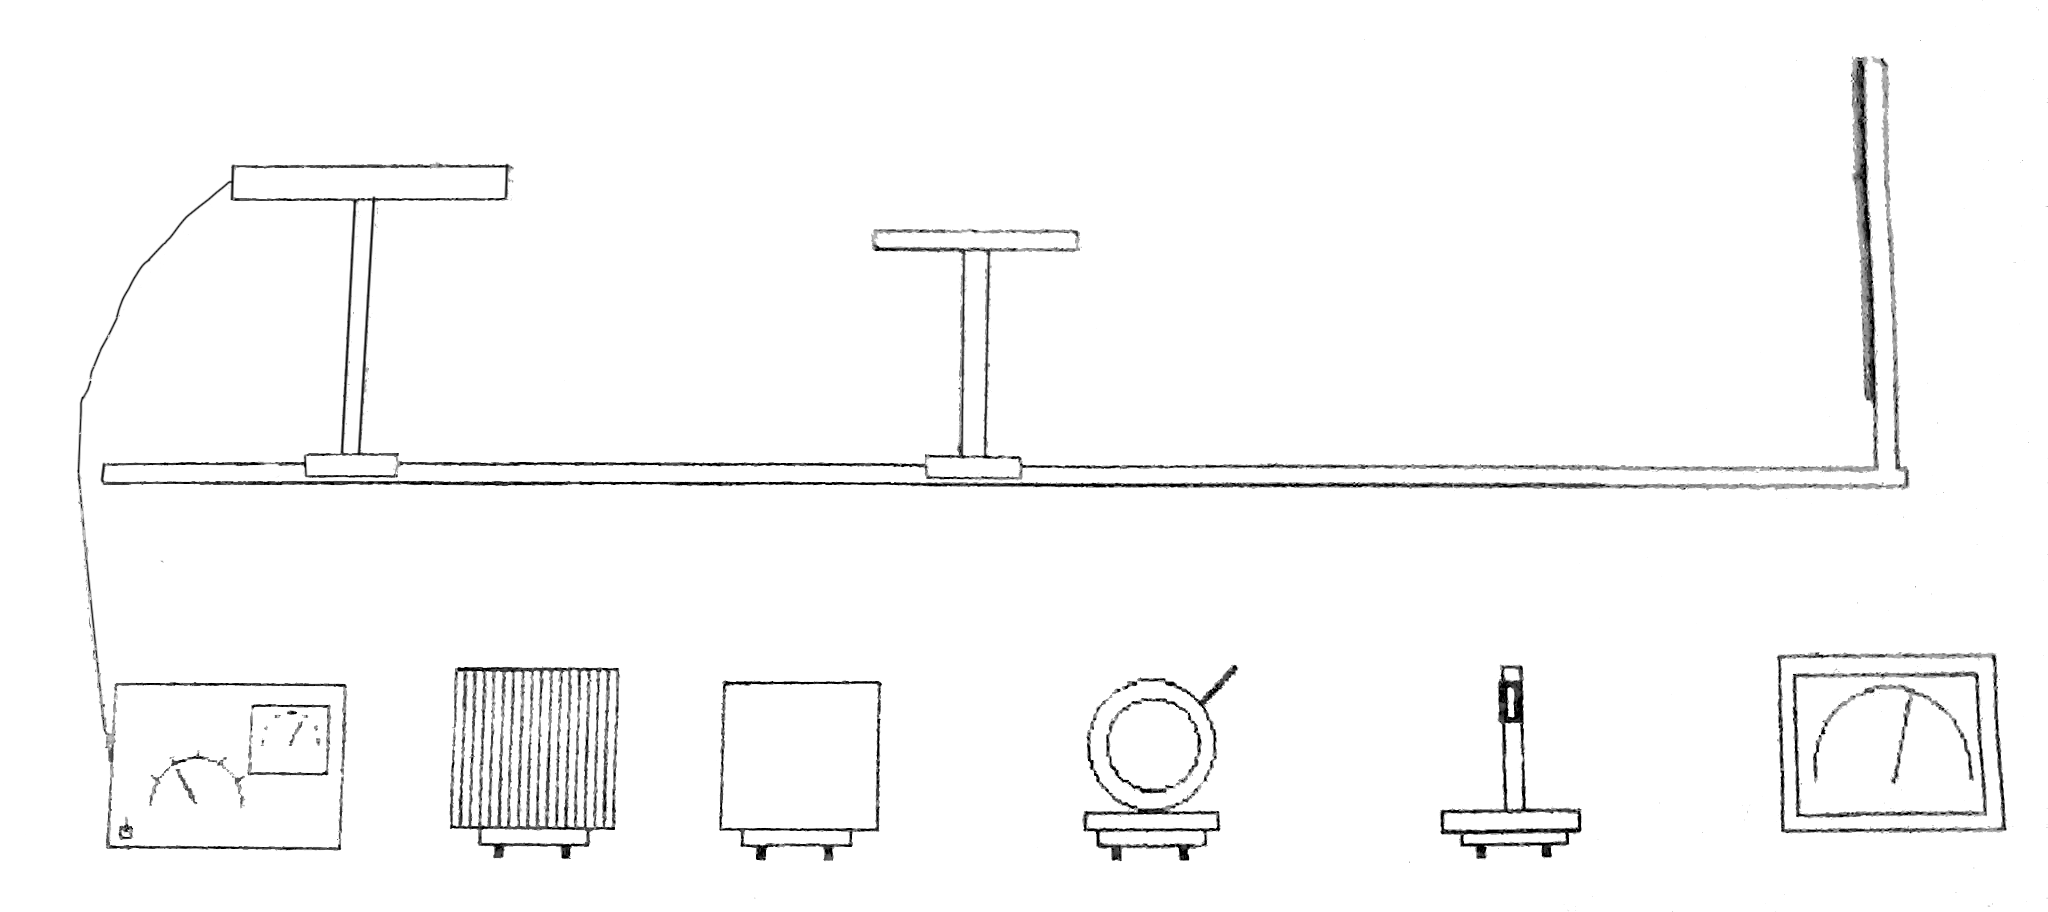
\includegraphics[width=.4\textwidth]{appearance}\\
        \parbox{.4\textwidth}{\caption{Внешний вид установки}}
    \end{figure}
    \vspace*{-2em}
    
    \begin{table}[h!]
        \center \caption{Определение длины волны излучения лазера}
        \begin{tabular}{|*{8}{C{.08}|}} \hline
            \( d \), мм & \( l \), мм & \( k \) & \( h \), мм &
                \( \phi \), град & \( \sin\phi \) & \( \lambda \), мм &
                \( \midnum{\lambda} \), мм \\ \hline
            \multirow{2}{*}{} & \multirow{2}{*}{} &&&&&&
                \multirow{2}{*}{} \\ \cline{3-7}
            &&&&&&& \\ \hline
            \multirow{2}{*}{} & \multirow{2}{*}{} &&&&&&
                \multirow{2}{*}{} \\ \cline{3-7}
            &&&&&&& \\ \hline
        \end{tabular}
    \end{table}
    
    \begin{table}[h!]
        \center \caption{Оценка направленности излучения лазера}
        \begin{tabular}{|*{7}{C{.08}|}} \hline
            & \( l \), мм & \( D_1 \), мм & \( D_2 \), мм & \( D_3 \), мм &
                \( \midnum{D} \), мм & \( \alpha \) \\ \hline
            1 & \multirow{2}{*}{} &&&&& \\ \cline{1-1}\cline{3-7}
            2 &&&&&& \\ \hline
        \end{tabular}
    \end{table}
    
    \begin{table}[h!]
        \center \caption{Наблюдение и подтверждение линейной поляризации
            излучения лазера}
        \begin{tabular}{|*{2}{*{3}{C{.08}|}|}*{3}{C{.08}|}} \hline
            \( \phi \) & \( I \) & \( I_1 \) &
                \( \phi \) & \( I \) & \( I_1 \) &
                \( \phi \) & \( I \) & \( I_1 \) \\ \hline
            0   && & 60  && & 120 && \\
            5   && & 65  && & 125 && \\
            10  && & 70  && & 130 && \\
            15  && & 75  && & 135 && \\
            20  && & 80  && & 140 && \\
            25  && & 85  && & 145 && \\
            30  && & 90  && & 150 && \\
            35  && & 95  && & 155 && \\
            40  && & 100 && & 160 && \\
            45  && & 105 && & 165 && \\
            50  && & 110 && & 170 && \\
            55  && & 115 && & 175 && \\
            180 && &&&&&& \\ \hline
        \end{tabular}
    \end{table}
    
    \pagebreak
    
    \subsection{Подсчет погрешности и окончательные результаты}
    \center
    \rule{.95\textwidth}{.5pt} \\ \rule{.95\textwidth}{.5pt}
    \rule{.95\textwidth}{.5pt} \\ \rule{.95\textwidth}{.5pt}
    \rule{.95\textwidth}{.5pt} \\ \rule{.95\textwidth}{.5pt}
    \rule{.95\textwidth}{.5pt} \\ \rule{.95\textwidth}{.5pt}
    \rule{.95\textwidth}{.5pt} \\ \vspace*{2em}
    
    \emph{Вывод:} \rule{.885\textwidth}{.5pt}
    \rule{.95\textwidth}{.5pt} \\ \rule{.95\textwidth}{.5pt}
\end{document}
